\chapter{State-of-the-art processor architectures}
The performance of a processor is defined by the the time it takes to execute a program. This time span, called \emph{\acsu{CPU} time}, can be expressed as:

\begin{equation*}
  \text{CPU time} = \frac{\text{Seconds}}{\text{Program}} = \frac{\text{Clock cycles}}{\text{Program}} \cdot T_{ck}
\end{equation*}
where $T_{ck}$ is the clock period.

The first term can be decomposed further by computing the total number of instructions inside a program, called \acfi{IC}, which is known given the assembly code of the program. From this figure and the total number of clock cycles, the average number of \acfi{CPI}\footnote{Sometimes, also the inverse figure can be used, that is \acfi{IPC}.} can be derived. By factoring in these quantities, the final expression of \ac{CPU} time is as follows \cite[p.~53]{hennessy17}:

\begin{equation}\label{eq:perf}
  \text{CPU time} = \text{IC} \cdot \text{CPI} \cdot T_{ck} 
\end{equation}

Equation \eqref{eq:perf} shows that the processor performance is directly and equally dependent on three factors:
\begin{itemize}
  \item Clock period, which depends mainly on the implementation technology and the microarchitectural choices (e.g. pipeline depth).
  \item \acsu{IC}, which is determined for the most part by the \ac{ISA} (see section \ref{sec:isas}) and compiler technology.
  \item \acsu{CPI}, which is dependant on both the \ac{ISA} and the architecture.
\end{itemize}
The goal is then to minimize each of these terms, but it is evident that none of these parameters can be modified without affecting the others, as many design choices influence many of them.

\section{Instruction-level parallelism}\label{sec:ilp}
Earliest processors executed instructions one at a time, fetching a new one only after the previous has finished, leading to a number of clock cycles per instruction greater than one, and in particular equal to the number of stages an instruction must get through. These processors, where $\text{CPI} > 1$, are called \emph{subscalar}. To illustrate the situation, in the example of the classic 5-stage RISC pipeline (fetch, decode, execute, memory access, write back), a subscalar processor would execute three consecutive instructions as shown in figure \ref{fig:subscalar}, taking a total of 15 clock cycles.

\begin{figure}[hbtp]
  \centering
  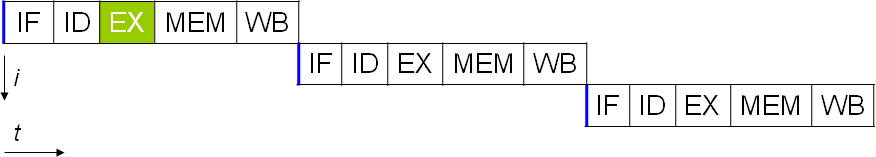
\includegraphics[width=0.8\textwidth]{img/subscalar.png}
  \caption{Subscalar processor}
  \label{fig:subscalar}
\end{figure}

Starting from the mid 80s, processor architects introduced \emph{pipelining} to improve performance by overlapping the execution of different instructions. This overlap means that at any given point in time there can be multiple instructions running in different stages of the processor, that is \emph{in parallel}, hence the term \acfi{ILP}\acused{ILP}, which is a fundamental concept in developing techniques to enhance processor performance. For the same example of figure \ref{fig:subscalar}, a pipelined processor could theoretically achieve a \ac{CPI} of 1, executing one instruction for each clock cycle (see figure \ref{fig:scalar}). Processors of this kind are called \emph{scalar}.

\begin{figure}[hbtp]
  \centering
  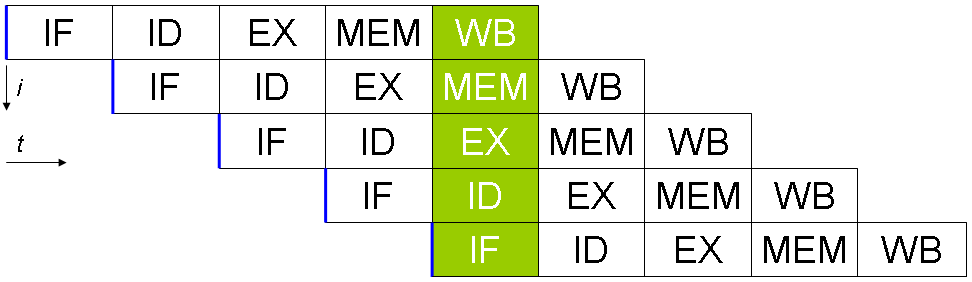
\includegraphics[width=0.8\textwidth]{img/scalar.png}
  \caption{Scalar processor}
  \label{fig:scalar}
\end{figure}

In practice however, data and control dependencies between successive instructions could cause hazards and force the pipeline to stall, causing CPI to rise once again at values greater than one. There are mainly three types of hazards that can take place in a pipelined processor:
\begin{itemize}
  \item \textbf{Structural hazards} arise when a hardware block is needed by two or more instructions at the same point in time. For instance, if a processor features only one memory block for both instructions and data, then two different instructions executing in the fetch and memory access stages could generate a structural hazard when trying to read from memory. Such hazards can either be easily solved (e.g. separate instruction and data memory in this example) or are known and accepted by the designers, given the limited hardware available.
  \item \textbf{Data hazards} in a simple pipelined processor occur when there is a \emph{data dependence} between instructions, that is one instruction needs to read a value that provided by a previous instruction. For example, in
      \begin{verbatim}
        add    x1,x2,x3
        sub    x4,x5,x1
      \end{verbatim}
      the \texttt{sub} instruction needs the value of register \texttt{x1} in the decode stage, but the previous \texttt{add} has not yet reached the write back stage and a data hazard is generated.
  \item \textbf{Control hazards} arise in the case of conditional flow changing instructions, such as branches, that prevent following instructions to be fetched until the new direction is resolved.
\end{itemize}

The real \ac{CPI} a pipelined processor can achieve is then given by the sum of the ideal \ac{CPI} and all the delays introduced by pipeline stalls caused by hazards \cite[p.~168]{hennessy17}:
\begin{equation}\label{eq:pipe_cpi}
  \begin{split}
    \text{CPI}  & = \text{Ideal CPI} + \text{Structural stalls} + \text{Data hazard stalls} + \text{Control stalls} \\
                & = 1 + \text{Structural stalls} + \text{Data hazard stalls} + \text{Control stalls} > 1
  \end{split}
\end{equation}

Those hazards become more frequent and more expensive to manage the more pipeline stages are introduced and that is a clear example of a tradeoff between two factors of the performance equation \eqref{eq:perf}: a deeper pipeline shortens the critical path and thus reduces the clock period, but at the same time it increases the CPI. That is the reason why designers at some point had to find other architectural solutions to improve performance.

\subsection{Multiple-issue processors}
A processor featuring a single execution pipeline can only achieve a theoretical \ac{CPI} of 1, but by duplicating the pipeline to include multiple execution units more than one instruction per clock cycle could be delivered. That is the idea that lies behind \emph{multiple-issue} processors, that exploit \ac{ILP} by executing independent instructions on separate execution pipelines.

Instructions that can be issued independently to the different pipelines are selected among a so called \emph{basic block}, that is a sequence of instructions comprised between single entry and exit points (i.e. with no branches or jumps in between). Recalling the examples of the previous section, figure \ref{fig:superscalar} shows the execution scheme for a multiple issue processor.

\begin{figure}[hbtp]
  \centering
  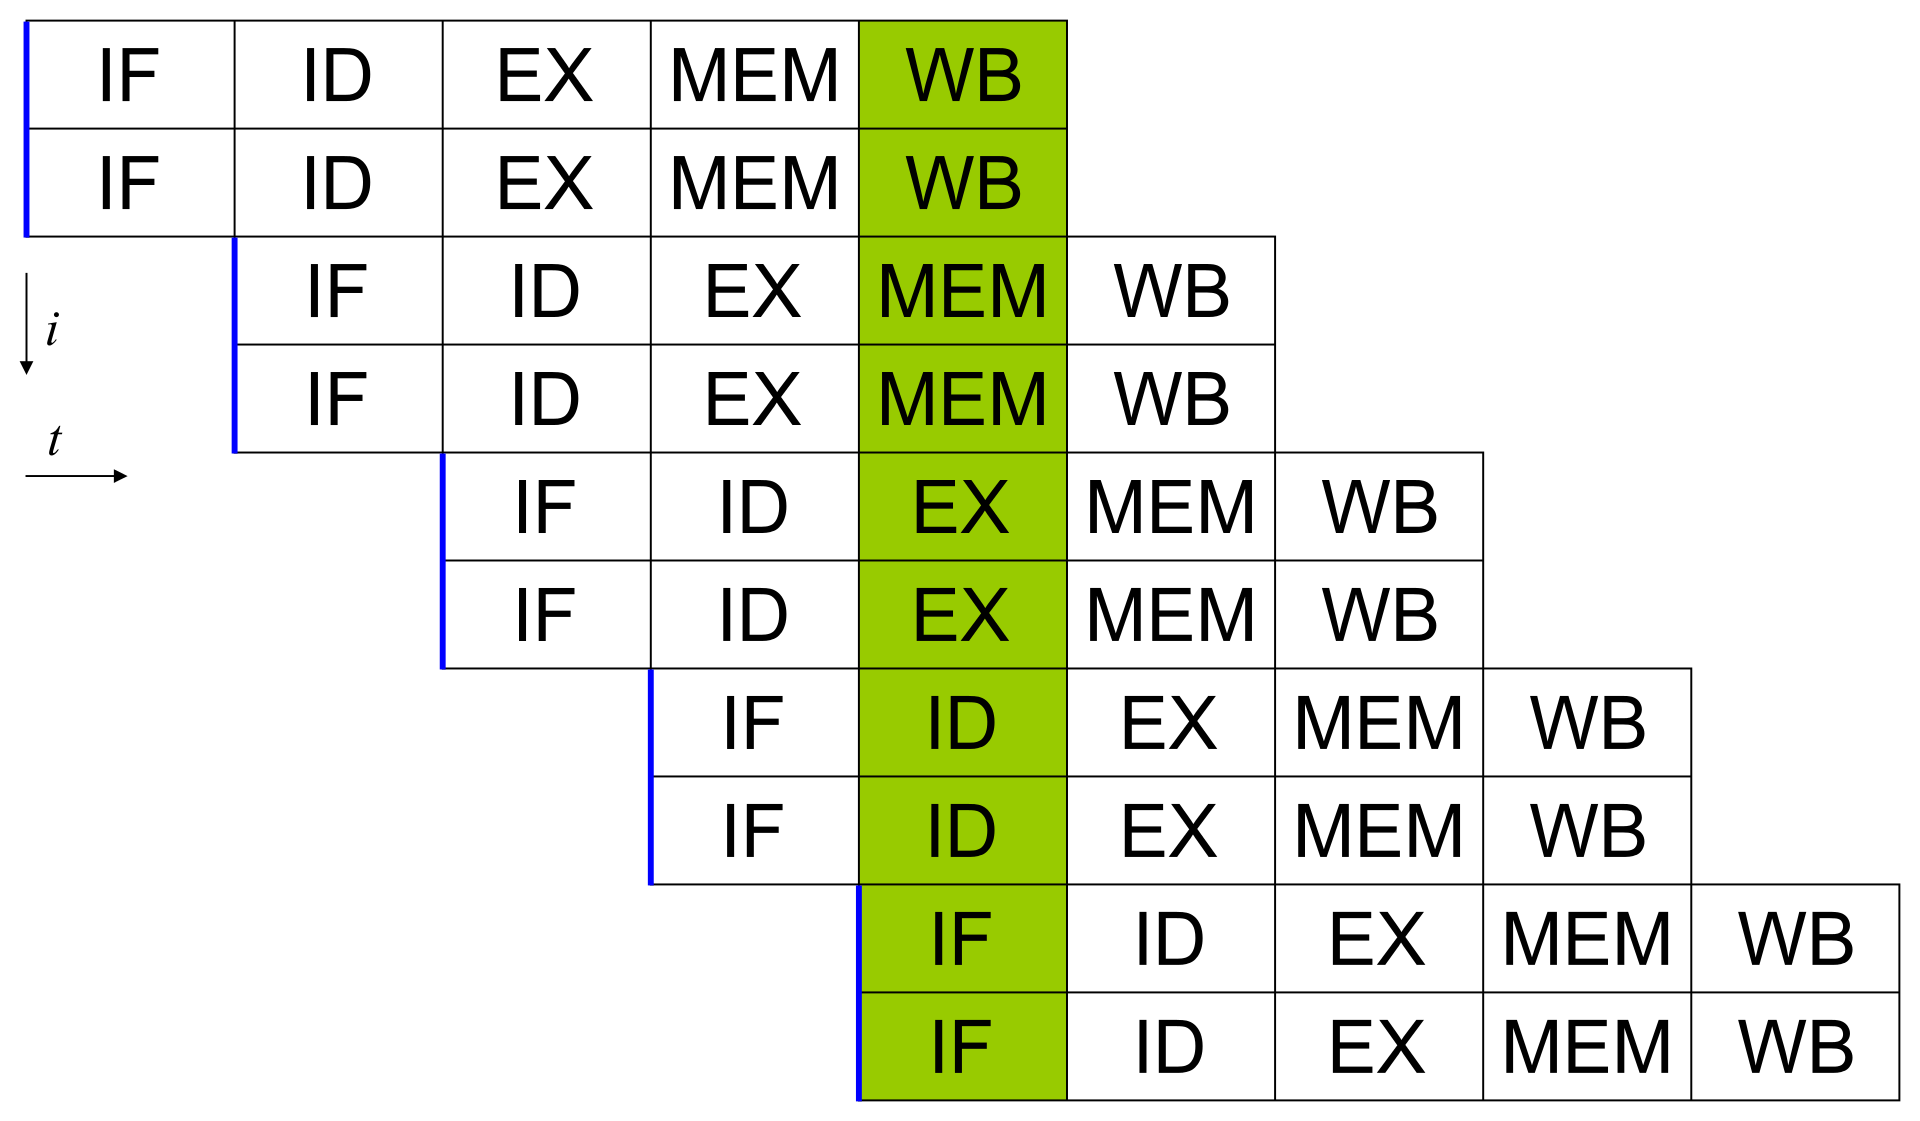
\includegraphics[width=0.8\textwidth]{img/superscalar.png}
  \caption{Multiple-issue processor with two pipelines}
  \label{fig:superscalar}
\end{figure}

Two main different approaches exist to multiple issue processors:
\begin{itemize}
  \item \textbf{\ac{VLIW}} processors, also known as \emph{static} multiple-issue, rely on software to discover \ac{ILP} chances at compile time, thus avoiding increased hardware complexity. The compiler groups instructions that can be executed in parallel in a single long packet-like instruction (hence the name \ac{VLIW}), that is then split and issued to the different execution units at run time. Despite many efforts, however, such static techniques reveal efficient only for specific applications presenting a high level of data parallelism \cite[p.~168]{hennessy17}, mainly because the compiler software needs a perfect knowledge of the underlying architecture in order to efficiently exploit \ac{ILP}.
  \item \textbf{Superscalar} processors, also known as \emph{dynamic} multiple-issue, on the other hand, rely on dedicated hardware to exploit \ac{ILP} at run time. Instructions belonging to a basic block are inserted into a \ac{WOE}, from where instruction that can run in parallel thanks to no data dependence are selected and issued to the respective following pipeline stages. This dynamic approach has been shown to work better than a static one, at the cost of a significant hardware complexity overhead.
\end{itemize}

Multiple-issue processors can achieve a \ac{CPI} lower than 1 (usually expressed at this point as \ac{IPC}, greater than 1) thanks to duplicate hardware units that also lower the impact of structural hazards, but they are nonetheless subject to data and control hazards. Instructions belonging to the same basic block are very likely to depend upon one another, as they are part of the same piece of program, and as such the amount of \ac{ILP} in contiguous instructions of a basic block is usually very small, leading to a low usage of the additional pipelines, and that is the reason why allowing multiple issues is not very useful by itself, but is almost always paired with the techniques analyzed in the next section.

\section{Dynamic scheduling}
All the processors seen in the previous sections adopted a so called \emph{static scheduling} of the pipeline, meaning that instructions are issued and executed along the pipe strictly in program order. To really extract the benefits of \ac{ILP}, however, all modern high-end processor employ a \emph{dynamically scheduled} pipeline, that can execute instructions out of order with respect to the assembled program. As an example consider the following code:
\begin{verbatim}
  add    x1,x2,x3
  sub    x5,x1,x4
  mul    x12,x18,x19
\end{verbatim}
In a classic 5-stage statically scheduled pipeline, instructions are executed in-order, and that means that the \texttt{mul} instruction cannot begin execution until the data dependence between \texttt{add} and \texttt{sub} is resolved by stalling the pipeline, as the execution takes place in program order. By using dynamic scheduling, on the other hand, if there are no structural hazards (and we can safely assume that that is the case, as the multiplier is likely to be a separate block from the \acsu{ALU}), the \texttt{mul} can be executed and maybe even completed before the \texttt{sub}. Instructions are then still issued in-order to the execution stage from the window of execution, but they can begin and complete execution \ooo.

Dynamic scheduling is almost always used in conjunction with superscalar processors, because the advantages given by the \ooo execution and the availability of multiple functional units go hand in hand. This combination offers several strengths compared to static scheduling or \ac{VLIW} processors \cite[p.~192]{hennessy17}. For instance, it allows compiled code to run in an efficient way on different microarchitectures, as the pipeline can manage itself and exploit \ac{ILP} without needing the help of the compiler. Moreover, it can handle cases where dependencies cannot be found at compile time, such as memory operations or dynamic branches. But the most important advantage of all is that an \ooo processor is able to mask the effect of unpredictable delays in the pipeline by executing later instructions without stalling. Remember that cache misses can easily take hundreds of clock cycles to resolve, which would turn into hundreds of wasted cycles in an in-order processor, but are instead taken advantage of to carry out unrelated tasks in an \ooo one.

In order to do so, the \ac{WOE} acts as a buffer between the fetch stages (called \emph{frontend}) and the execution and commit stages (called \emph{backend}), that hopefully always contains enough instructions to ensure a constant flow to the functional units, even when earlier instructions are waiting for some event. This is obviously possible only if the frontend is able to maintain a high enough bandwidth of fetched instructions to the \ac{WOE}.

\subsection{Dependencies and hazards}
Out-of-order processors are subject to all the dependencies listed in section \ref{sec:ilp}, but due to the reordering of instructions, other hazards can arise from so called \emph{name dependencies}. In this context, a useful taxonomy to categorize such hazards is defined\footnote{Structural and control hazards are not considered here, as they are the same as in an in-order processor.}. Let $D(i)$ be the \emph{domain} and $R(i)$ be the \emph{range} of instruction $i$, meaning respectively the registers or memory locations read and written by instruction $i$, and consider two instructions $i$ and $j$, with $j$ following $i$ in the program order. Then, there are three possible kinds of data hazards:
\begin{itemize}
  \item \textbf{\ac{RAW}} hazards are the only true data hazards arising from a data dependence and occur, as seen previously, when instruction $j$ is trying to read a piece of data before $i$ writes it, leading to a wrong value read by $j$, as in the following example:
      \begin{verbatim}
        add    x1,x2,x3
        sub    x4,x5,x1
      \end{verbatim}
      More formally, \ac{RAW} hazards occur if:
      \begin{equation*}
        R(i) \cap D(j) \neq \varnothing
      \end{equation*}
  \item \textbf{\ac{WAR}} hazards arise from the name dependence called \emph{anti-dependence}, that occurs when instruction $j$ writes the same location that $i$ reads, causing $i$ to read the wrong value if $j$ is executed first, as in:
      \begin{verbatim}
        add    x1,x2,x3
        mul    x2,x5,x6
      \end{verbatim}
      More formally, \ac{WAR} hazards occur if:
      \begin{equation*}
        D(i) \cap R(j) \neq \varnothing
      \end{equation*}
  \item \textbf{\ac{WAW}} hazards arise from the name dependence called \emph{output dependence}, that occurs when instructions $i$ and $j$ write their outputs on the same storage locations, leaving the final wrong value written by $i$, if $j$ is executed first, like in the following:
      \begin{verbatim}
        add    x1,x2,x3
        mul    x1,x5,x6
      \end{verbatim}
      More formally, \ac{WAW} hazards occur if:
      \begin{equation*}
        R(i) \cap R(j) \neq \varnothing
      \end{equation*}
\end{itemize}

It is hopefully clear that \ac{WAR} and \ac{WAW} hazards occur only in dynamically scheduled processors where instruction order can be rearranged and that the dependencies that cause them are called name dependencies, because it is only a matter of storage location used and not an issue with the correct outcome of the program. In the examples above, if the \texttt{mul} instruction could (temporarily) write its output on a different register, until the \texttt{add} completes, then the semantics of the program would respected and the hazards resolved without stalling. That is the idea that lies behind \emph{register renaming}, which is the technique used in \ooo processors at the decode stage to detect and solve \ac{WAR} and \ac{WAW} hazards by converting the architectural registers that instructions refer to to different physical registers hidden to the programmer and compiler.

\subsection{Scheduling techniques}
Out-of-order execution needs dedicated hardware to select instructions inside the \ac{WOE} and detect and prevent hazards. For this purpose, several schemes and algorithms exist, among which are \emph{scoreboarding} and \emph{Tomasulo's algorithm} that are described in the following.

\subsubsection{Scoreboarding}
Scoreboarding is a centralized scheduling technique first introduced in the CDC 6600 in the 60s \cite{scoreboard} and still widely used today. The algorithm provides the following stages for each instruction after the decoding:
\begin{itemize}
  \item \textbf{Issue}: instructions stall in this stage until there are no structural hazards and all the output dependencies with previously issued instructions are resolved, to avoid \ac{WAW} hazards.
  \item \textbf{Read operands}: instructions can proceed when their operands are available, resolving \ac{RAW} hazards, in an \ooo fashion.
  \item \textbf{Execute}: operands are passed to the functional units that perform the requested operations.
  \item \textbf{Write result}: the write back operation is stalled until all earlier instructions that are anti-dependent have read the previous value, resolving \ac{WAR} hazards. 
\end{itemize}

Each of these stages can take an arbitrary number of cycles, thus, in order to control the progress of all instructions, a set of three data structures is used as shown in figure \ref{fig:scoreboard}.
\begin{figure}[hbtp]
  \centering
  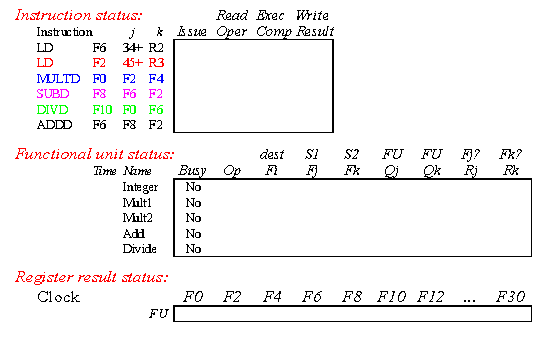
\includegraphics[width=0.8\textwidth]{img/scoreboard.pdf}
  \caption{Scoreboard structure}
  \label{fig:scoreboard}
\end{figure}
The first one is the \emph{instruction status} table, that keeps track of which of the four stages each instruction is currently in. Then, there is the \emph{functional unit status} table, which has nine fields for each functional unit, indicating if that unit is busy, what operation it has to perform, the destination register, the source operands registers, the functional units that will produce the operands and two flags indicating when those operands are ready. Finally, the \emph{register result status} table indicates for each register which functional unit will write its result to it.

The original scoreboarding algorithm did not include register renaming and so \ac{WAW} and \ac{WAR} hazards could potentially cause the pipeline to stall in the issue and write result stages respectively. For this reason, register renaming can still be implemented, but it must be carried out in the issue stage, by a dedicated renaming unit, like the one shown in figure \ref{fig:renaming}, based on the one included in the MIPS 10000.
\begin{figure}[hbtp]
  \centering
  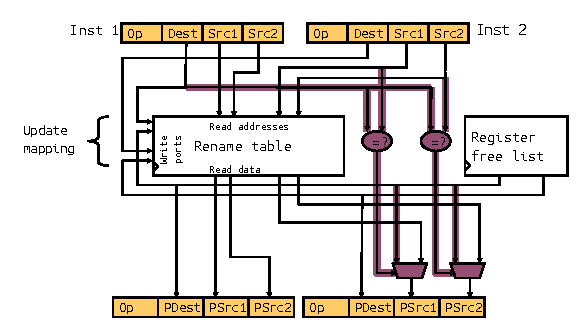
\includegraphics[width=0.9\textwidth]{img/renaming.pdf}
  \caption{Renaming unit}
  \label{fig:renaming}
\end{figure}
The \emph{rename table} keeps track of the mapping between architectural and physical registers, to maintain correct value references, while the \emph{register free list} contains the names of all available physical registers to be used for renaming. As this unit renames two instructions in parallel, it has to check for \ac{RAW} hazards between them, and in case there is one, rename the second instruction with the newly assigned physical registers to the other one. 

Using this scheme, also known as \emph{explicit} register renaming, \ac{WAW} and \ac{WAR} hazards are completely avoided as early as an instruction is decoded and issued, meaning that no further checks must be performed in the later stages of the algorithm.

\subsubsection{Tomasulo's algorithm}
Invented by Robert Tomasulo for the IBM 360/91 \ac{FPU}, this algorithm offers a different approach to dynamic scheduling, by adopting a \emph{distributed} control instead of a centralized one, as present in scoreboarding. This idea is based around the concept of \emph{reservation stations}, which are buffers placed in front of each functional unit, including load and store units, to store instruction operands. A generic architecture based on Tomasulo's approach is shown in figure \ref{fig:tomasulo}.
\begin{figure}[hbtp]
  \centering
  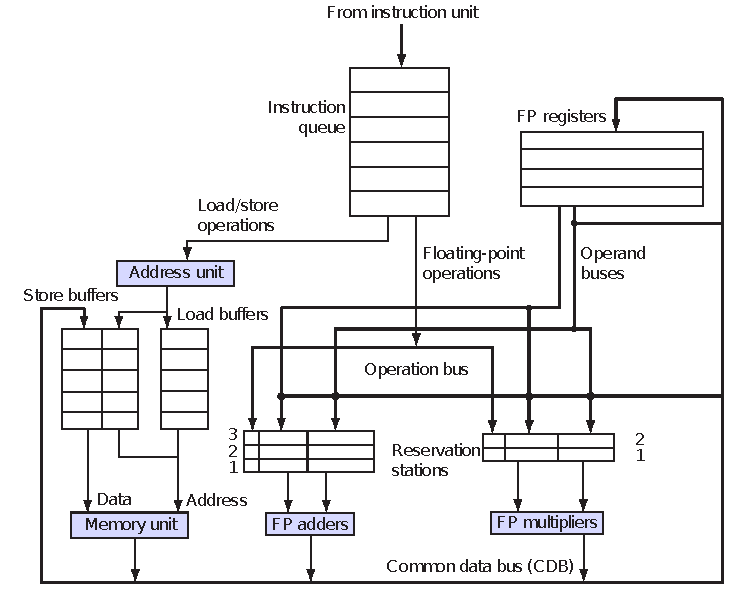
\includegraphics[width=0.9\textwidth]{img/tomasulo.pdf}
  \caption{\acs{FPU} example architecture using Tomasulo's algorithm \cite[p.~198]{hennessy17}}
  \label{fig:tomasulo}
\end{figure}

Each reservation station contains several fields providing similar information with respect to functional unit status data structure used in scoreboarding: which operation to perform, the reservation stations from which the source operands will come, the value of the operands and the busy status. The key difference with scoreboarding is, however, that the results of the functional units are broadcast to the register file as well as to all the reservation stations through a \ac{CDB}, while the scoreboarding technique only writes results to registers. This, in turn, provides the great advantage of allowing \emph{implicit} register renaming at each reservation station, because register names are discarded when an instruction is issued to a reservation station, as operands will come from another reservation station of from the \ac{CDB} as soon as they become available. Moreover, if multiple instructions are waiting on the same result, they can all be started simultaneously when such result arrives because of the presence of multiple reservation stations, while on the other hand, using scoreboarding, they would wait in turn for the register file bus to be free, possibly wasting clock cycles \cite[p.~201]{hennessy17}.

In the end, the steps that each instruction must get through are similar to the one in scoreboarding, but the actions performed are different:
\begin{itemize}
  \item \textbf{Issue}: instructions are fetched in-order from the issue queue stall in this stage until there is a matching reservation station available (no structural hazards) and then are issued to the reservation station with implicit renaming.
  \item \textbf{Execute}: the \ac{CDB} is monitored until all operands are available (avoid \ac{RAW} hazards), at which point the functional unit executes the instruction.
  \item \textbf{Write result}: as soon as an operation completes, the result is written on the \ac{CDB} and from there to the register file and reservation stations.
\end{itemize}

Tomasulo's algorithm is today used in many high-performance processors and it has been chosen also for the design of LEN5.

\section{Hardware-based speculation}
For typical \acp{ISA} around 10--20\% of instructions are branches, meaning that an average basic block will not contain more than 5 to 10 instructions. This is obviously a significant constraint, as the amount of \ac{ILP} that can be exploited in such a small set of instructions without incurring in control dependencies is quite limited. From these reason the idea of \emph{hardware-based speculation} was born, based on three principles \cite[p.~208]{hennessy17}:
\begin{itemize}
  \item Dynamic branch prediction, to fetch and issue instructions before the outcome of a branch is determined (refer to section \ref{sec:dynbp} for details).
  \item Speculative execution, to allow the execution of such instructions even if their control dependencies are not resolved yet.
  \item Dynamic scheduling, to schedule instructions crossing the boundary of a single basic block.
\end{itemize}

This represents an important improvement over mere dynamic scheduling and even branch prediction alone, because this way instructions are executed as if the guesses on the taken direction were always correct, leading to a \emph{data flow execution} of the program, where operations are executed as soon as their operands are available, irrespective of control flow.

Of course, some precautions must be taken in order to handle the situation when the speculated flow was predicted incorrectly, as to restore the original state of the processor and proceed down the right path. For this reason, an additional stage after the write result must be inserted in order to decouple the production of a result by a functional unit and the actual irreversible update of the register file and data memory, that can take place only when an instruction is no longer speculative. This last step is called \emph{instruction commit} and must always be performed in-order.

\subsection{\acl{ROB}}
In both scoreboarding and Tomasulo's approach, instruction commit can be handled using a dedicated hardware structure called \ac{ROB}. As the name implies, the \ac{ROB} acts as a buffer between the functional unit outputs and the register file and memory, storing speculative results until the speculation is resolved and thus effectively increasing the number of registers available, similarly to reservation stations. A general scheme of an architecture using the \ac{ROB} is shown in figure \ref{fig:robpipe}, highlighting which parts of the pipeline are in-order and which \ooo.
\begin{figure}[hbtp]
  \centering
  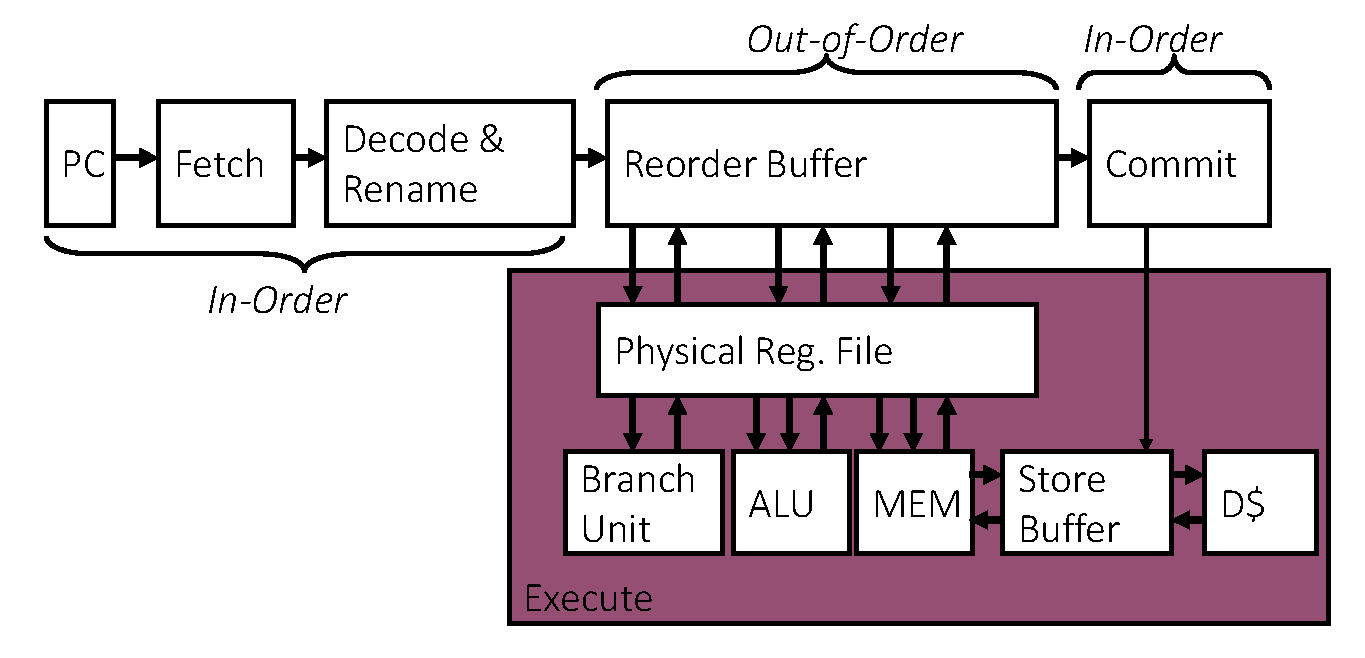
\includegraphics[width=0.8\textwidth]{img/robpipe.pdf}
  \caption{An \ooo pipeline featuring register renaming and \acs{ROB}}
  \label{fig:robpipe}
\end{figure}

\subsubsection{\acs{ROB} with Tomasulo's algorithm}
As stated above, the \ac{ROB} extends the number of available registers and thus provides renaming on its own by substituting the register file before instruction commit. Moreover, alongside the reservation stations and the \ac{CDB}, the \ac{ROB} serves as another source of operands, as figure \ref{fig:robtomasulo} shows. Finally, for its intrinsic nature, the \ac{ROB} also serves almost the same purpose of the store buffer as a reservation station before the data memory.
\begin{figure}[hbtp]
  \centering
  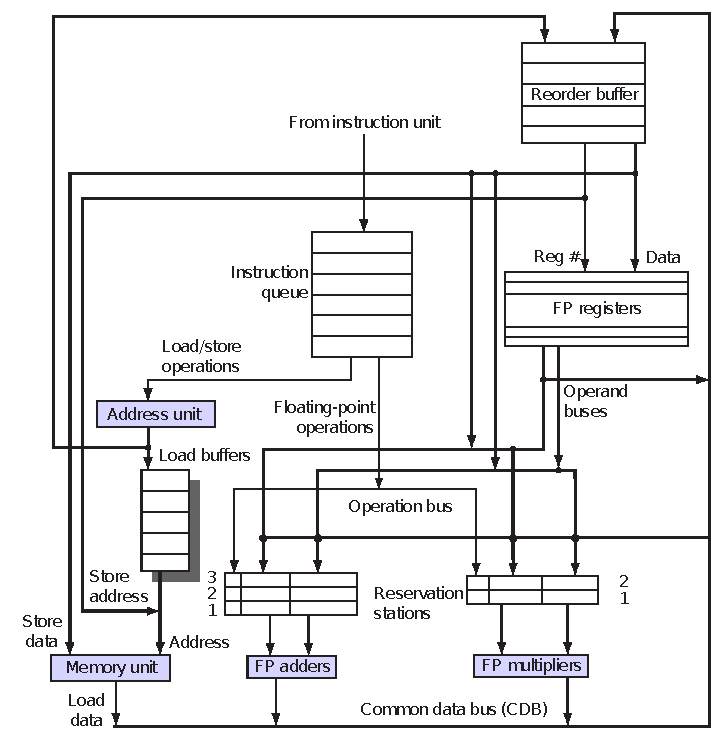
\includegraphics[width=0.8\textwidth]{img/robtomasulo.pdf}
  \caption{\acs{FPU} example architecture using Tomasulo's algorithm and \acs{ROB} \cite[p.~210]{hennessy17}}
  \label{fig:robtomasulo}
\end{figure}

In terms of algorithm steps, what changes is that during execution the results are broadcast on the \ac{CDB} and to the \ac{ROB} instead of to the register file. In addition, during the added step of instruction commit, an instruction is removed when it reaches the head of the \ac{ROB} (which acts as a circular buffer) and, if it is a branch with a wrong prediction to reach the commit stage, then the \ac{ROB} gets flushed and execution resumes at the correct target of the branch.

\section{Summary of \acs{ILP} techniques}
To summarize this overview of multiple-issue processors and techniques to exploit \ac{ILP}, table \ref{tab:multissue} provides all the important differences at a glance.
\begin{table}[hbtp]
  \centering
  \rowcolors{1}{}{gray!10}
  \makebox[\textwidth][c]{
    \begin{tabular}{p{\dimexpr 0.16\linewidth}
                    p{\dimexpr 0.13\linewidth}
                    p{\dimexpr 0.13\linewidth}
                    p{\dimexpr 0.14\linewidth}
                    >{\raggedright}p{\dimexpr 0.18\linewidth}
                    >{\raggedright\arraybackslash}p{\dimexpr 0.22\linewidth}}
      \toprule
      \textbf{Name} & \textbf{Issue structure} & \textbf{Hazard detection} & \textbf{Scheduling} & \textbf{Relevant features} & \textbf{Examples} \\ \hline
      Superscalar (static) & Dynamic & Hardware & Static & In-order    execution & Embedded MIPS and ARM cores \\
      Superscalar (dynamic) & Dynamic & Hardware & Dynamic & Out-of-order execution, but no speculation & None \\
      Superscalar (speculative) & Dynamic & Hardware & Dynamic & Out-of-order execution and speculation & Intel Core i3, i5, i7, AMD Ryzen \\
      \ac{VLIW} & Static & Software & Static & Hazards detected by the compiler & Signal processors like the TI C6x \\
      \bottomrule
    \end{tabular}
  }
  \caption{Summary table of multiple-issue approaches \cite[p.~219]{hennessy17}}
  \label{tab:multissue}
\end{table}